\documentclass[12pt]{article}
\usepackage{amsmath} % flere matematikkommandoer
\usepackage[utf8]{inputenc} % æøå
\usepackage[T1]{fontenc} % mere æøå
\usepackage[danish]{babel} % orddeling
\usepackage{verbatim} % så man kan skrive ren tekst
\usepackage[all]{xy} % den sidste (avancerede) formel i dokumentet
\usepackage{graphicx}
\usepackage{listings}
\usepackage{url}
\title{ProjektKursus Systemudvikling 2014\\Delrapport 4}
\author{}

\begin{document}
\maketitle
\noindent{Gruppemedlemmer:}\\
Kenneth Christensen: 02 08 93\\Michael Jensen: 01 07 93\\Rune Pedersen: 01 11 82\\Rasmus Hansen: 03 12 92
\\\\
Instructor: Kasper Passov

\pagebreak
\tableofcontents
\pagebreak
\section{Abstract}
We have choosen to work on a project for a local bike shop called "bmx-butikken". Bmxbutikken is specialised in the freestyle BMX community. They sell all you need as a BMX rider, which is everything from cloths and shoes to complete bikes and parts. They have a phsyical shop on Nørrebrogade, and a webshop at \url{www.bmxbutikken.dk}. The project regards a Spotguide app for all devices, programmed as a web application. This site is supposed to help local riders to find new places to ride, and foreigners to find any places to ride and hook up with the local crew. The app can also show you where bmx-butikken is located if you need a spare part. The application is designed for all bmx riders mainly in Copenhagen, but spots can be uploaded from anywhere.

\pagebreak 

\section{IT-projektets formål og rammer}
Følgende model er en FACTOR analyse af projektet og giver en kort og konkret beskrivelse af rammerne for projektet. Modellen er udarbejdet efter inspiration fra et uddrag af Oriented Analysis og Design (2.7 The FACTOR Criterion).\\\\
F - Functionality: beskriver hvilke værktøjer og funktionaliteter kunden får igennem appen.\\
A - Application Domain: beskriver hvem vi prøver at ramme med projektet og altså hvem der vil have gavn af vores arbejde.\\
C - Conditions: beskriver hvilke krav der er til kørsel af projektet (applikationen), det være sig brugerens udstyr samt appens tilgængelighed.\\
T - Technology: beskriver hvilke udviklings værktøjer vi vil gøre brug af undervejs i projektet.\\
O - Objects: indeholder de objekter vi arbejder med. Disse objekter er en del af løsningen til problemområdet.\\
R -Responsibilities: Hvad er applikationens rolle, pligter og hvad er den grundlæggende løsning til problemet.\\


\begin{raggedleft}
  \begin{tabular}{| l | l |}
    \hline
    Funktionalitet & Give oplysninger om bmx spots\\ & Give oplysning om specialiserede bmx butikker\\ & Give rutevejledning\\ \hline
    Application Domain & BMX udøverer og bmxbutikkens kunder\\ \hline
    Conditions & Hjemmesiden skal kunne køres på smartphones\\ & Åben internet forbindelse \\ & Adgang til din lokation\\
    \hline
        Technology & HTML \\ & Javascript \\ & CSS\\ & mySQL\\ & PHP\\
    \hline
        Objects & Skate Spots\\ & Shops\\ & BMX Spots\\
    \hline
        Responsibilities & Give information om spots\\ & Informerer om selve bmxbutikken\\
    \hline
  \end{tabular}
\end{raggedleft}


\pagebreak

\section{Kravspecifikation for IT-løsningen}
I denne sektion beskriver vi hvad der er funktionelle og ikke-funktionelle krav.\\
De \textbf{funktionelle krav }beskriver hvad i systemet der kræver deciderede funktioner der modellerer med vores database. Altså hvordan system skal virke. Dette er vigtigt da de netop fortæller om funktioner der skal være i systemet og giver et indblik i strukturen.\\
De \textbf{ikke funktionelle krav} specificerer de krav der er for systemet der ikke har en direkte indvirkning op programmet. Dog er de en vigtig faktor da det er disse der er er med til at skabe interfacet, altså hvordan det ser ud og hvordan det føles at navigere igennem det hele. Altså det hvordan de vil vise det systemet gør.\\ 
\textbf{Constraints} er hvilke begrænsninger vi har på vores system, altså hvordan tingene skal være opbygget. Disse er med til at danne en mindre struktur over hvad der er meget vigtigt for vores system.
\subsection*{Funktionelle krav}
\textbf{Add spot} \\ Gør det muligt for en bruger at tilføje nye spots til kortet. Dette er til for at kortet hele tiden kommer til at udvide sig med diverse nye spots som brugerne kan finde og dele med andre. Det fungerer sådan at man udfylder en formular med lokalitet og beskrivelse og man har samtidig mulighed for at uploade billeder. Dette er et krav idet at der vil dukke nye og spændende spots op og appen skulle helst være op to date\\
\textbf{Settings}\\ Gør det muligt at bestemme hvor stor en radius man vil se spots i udfra ens egen lokation. Dette er især vigtigt hvis man rejser på cykel og gerne vil begrænse hvor langt man skal rejse.\\
\textbf{Search}\\ Gør det muligt for brugeren at finde et specifikt spot udfra dens navn. Så det bliver nemmere og hurtigere for brugeren at finde lige det spot han/hun leder efter.\\
\textbf{Streetspots}\\ Viser brugeren en liste over de forskellige spots med billede. Dette er til for hvis brugeren ikke vil se diverse spots på kortet, men finder det mere overskueligt at se det på en liste.\\
\newpage
\noindent{\textbf{Markers}}\\ Viser på kortet 3 ting: Brugerens lokation, diverse spots og bmxbutikkens lokation. Disse markers er nødvendige for at man kan se spots'ne på kortet.\\
\textbf{Bruger lokation}\\ Finder brugerens lokation. Er nødvendig i forhold til at beregne forskellige funktioner ud fra brugerens placering\\
\textbf{Shops}\\ Skal vise en liste over de shops der er tilknyttet projekt(pt er dette dog kun en butik). Er et krav idet at der ønskes at brugerne er opmærksomme på at de pågældende butikker findes og hvor de er.
\subsection*{Ikke funktionelle krav:}
\textbf{Sprog}\\ Siden skal være på engelsk, så den kan bruges af turister, men samtidig også af de lokale da de fleste i miljøet snakker engelsk.\\
\textbf{Menu}\\ Der skal være en menu der indeholder 5 ting du kan trykke på der kan vejlede bruger: Spots, shops, settings, Add spot, Search\\
\textbf{Usability}\\ Skal være til at bruge af alle at brugerer. Nemt og intuitivt at finde rundt i.
\textbf{Reliability}\\ Skal være oppe og klar til brug, altid.\\
\textbf{Performance}\\ Skal kunne holde til så mange brugere som muligt, altså ikke begrænse hvor mange der kan være på samtidigt med det fungerer hurtigt. \\
\textbf{Farve af Markers}\\ De forskellige typer af markers skal have forskellige farver så brugeren nemmere kan overskue det.
\subsection*{Constraints}
Systemet skal være kompatibelt med både computere og telefoner.[Implementation requirement]\\
Kortet skal vise en marker ved bmxbutikken[User Interface Requirement]\\
Koden skal være skrevet i php/javascript/html/mysql.[Implementation requirement]\\

\pagebreak
\section*{Use-cases}
\subsection*{Use-case model}
\begin{figure}[htb]
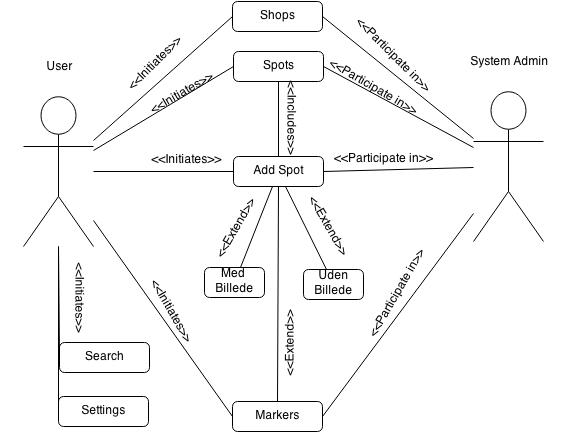
\includegraphics[scale = 0.8]{UM.jpg}
\end{figure}

Højniveau diagram der skal illustrere de forskellige aktører\\\\
\newpage
\noindent Som det ses er der 2 aktører, brugeren og System administratoren. Brugeren benytter appen og det er altså brugeren der "initiates" eller starter en given funktion, det være sig: At klikke på Add Spot og tilføje et spot uden billede eller at ændre indstillingerne. Som det ses på modellen er alle funktioner brugeren har adgang til og brugeren selv forbundet.\\\\ Derudover har enkelte funktioner noget med hinanden at gøre. Som det ses er "Add Spot" forbundet med Markers, Spots, Med billede og uden billede. Dette er fordi at man både kan tilføje nye spots uden eller med billeder. Samtidig er det disse spots der kommer frem på kortet som "Markers" og det nye spot bliver inkluderet under den generelle mappe for "Spots".\\\\
Til sidst er der System administratoren som er forbundet med Shops, Spots, Add Spot og Markers. Dette skyldes at System Administratoren er med til at opdatere de givne funktioner.

\pagebreak
\setlength\parindent{0pt}
\subsection*{Få information om et spot}
\hrule\vspace{5mm}
\textit{Use case name:} FindSpot\\
\hrule\vspace{5mm}
\textit{Actor:} en bruger der gerne vil finde information om et spot\\
\hrule\vspace{5mm}
\textit{Entry condition:} brugeren åbner appen\\
\hrule\vspace{5mm}
\textit{Flow of events:}
\begin{enumerate}
\item Brugeren bliver præsenteret for et kort med sin egen positition i centrum og en menu linje i toppen
\item Brugeren trykker på en "marker" på kortet for det spot han vil se information.
\end{enumerate}
\hrule\vspace{5mm}
\textit{Exit condition:} Brugeren ser nu et pop-up vindue med information om spottet.\\
\hrule\vspace{5mm}
Dette use-case beskriver en bruger som gerne vil have nogen information om et specifikt spot. Brugeren åbner app'en på 
sin telefon og bliver præsenteret med kort-interfacen. Kort-interfacen er kort over brugerens position med en menu-bar 
i toppen. På kortet vil der være faner som repræsenteret spots. Bruger trykker på fanen for det spot han gerne vil have
informationer og app'en viser så disse information i et pop-up vindue henover kortet.
\newpage
\subsection*{Tilføj spot}
\hrule\vspace{5mm}
\textit{Use case name:} AddSpot\\
\hrule\vspace{5mm}
\textit{Actor:} en bruger der gerne vil tilføje et spot\\
\hrule\vspace{5mm}
\textit{Entry condition:} brugeren åbner appen\\
\hrule\vspace{5mm}
\textit{Flow of events:}
\begin{enumerate}
\item Brugeren trykker på knappen "Add spot", der sender ham videre til en udfyldelses formular
\item Brugeren udfylder formularen og gemmer denne, formularen sendes derefter til godkendelse hos administratoren
\end{enumerate}
\hrule\vspace{5mm}
\textit{Exit condition:} Brugeren sendes retur til forsiden\\
\hrule\vspace{5mm}
Dette use-case beskriver en bruger som gerne vil tilføje et spot til app'en. Brugeren åbner app'en på sin telefon og 
bliver præsenteret med kort-interfacen. Kort-interfacen er kort over brugerens position med en menu-bar i toppen. Brugeren
trykker på "Add spot" knappen i menuen og bliver herefter præsenteret med en formular som skal udfyldes. Denne formular 
består af tekst-felter samt muligheden for at tilføje et billed. Brugeren udfylder formularen og submiter den, hvorefter
brugeren bliver returneret til kort-interfacen.
\newpage
\subsection*{Ændre indstillinger}
\hrule\vspace{5mm}
\textit{Use case name:} ChangeCondition\\
\hrule\vspace{5mm}
\textit{Actor:} en bruger der gerne vil ændre indstillingerne\\
\hrule\vspace{5mm}
\textit{Entry condition:} brugeren åbner appen\\
\hrule\vspace{5mm}
\textit{Flow of events:}
\begin{enumerate}
\item Brugeren trykker på indstillinger, der sender brugeren videre til en ny side
\item Brugeren bliver præsenteret for de forskellige indstillinger han kan vælge
\item Når brugeren han ændret indstillinger er der en ok knap som tilføjer indstillingerne
\end{enumerate}
\hrule\vspace{5mm}
\textit{Exit condition:} Indstillingerne er nu i funktion og brugeren sendes tilbage til forsiden\\
\hrule\vspace{5mm}
Dette use-case beskriver en bruger som gerne vil ændre den radius som app'en loade spots fra. Brugeren åbner app'en på 
sin telefon og bliver præsenteret med kort-interfacen. Kort-interfacen er kort over brugerens position med en menu-bar i 
toppen. Brugeren vælger indstillinger fra menuen og bliver præsenteret med slider-bar. Brugeren vælger den ønsket radius
og trykker "accept". Bruger bliver herefter returneret til kort-interfacen.
\pagebreak

\subsection*{Klassediagram}
\begin{figure}[h]
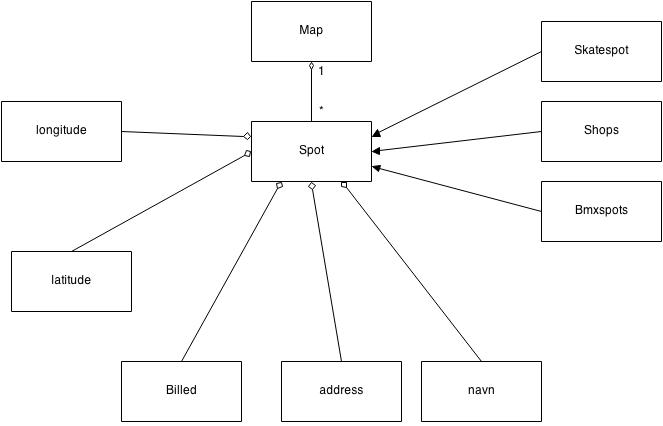
\includegraphics[scale = 0.5]{classdiagram}
\end{figure}
Klasse diagrammet viser systemets opbygning:
Vi har et kort, dette kort har et "et-til-mange" forhold til vores spots.
Disse spots kan være af tre typer: Bmx-spots, skate-spots og shops.
Disse tre nedarver fra "spots" som har nogle attributer. Disse attributer er : Latitude, longitude, addresse, navn og muligvis et billed.
\newpage
\subsection*{Sekvensdiagram over find spot information}
\begin{figure}[h]
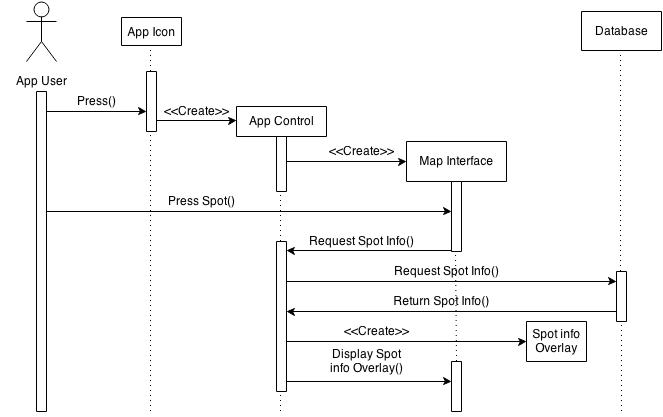
\includegraphics[scale = 0.5]{sekdia1}
\end{figure}

Brugeren starter App'en, ved at trykke på iconet for App'en, på sin telefon. App'en viser kort interfacen, 
som er et kort over brugerens nuværende position med en menu-bar i toppen. Spotsne vil blive repræsenteret 
på kortet i form af faner. Brugeren vælger et spot fra kortet ved at trykke på en fane. App'en henter
informationerne om spottet, fra database, og viser dem i et overlay hen over kortet.
\newpage

\subsection*{Sekvensdiagram over add spot funktionen}
\begin{figure}[h]
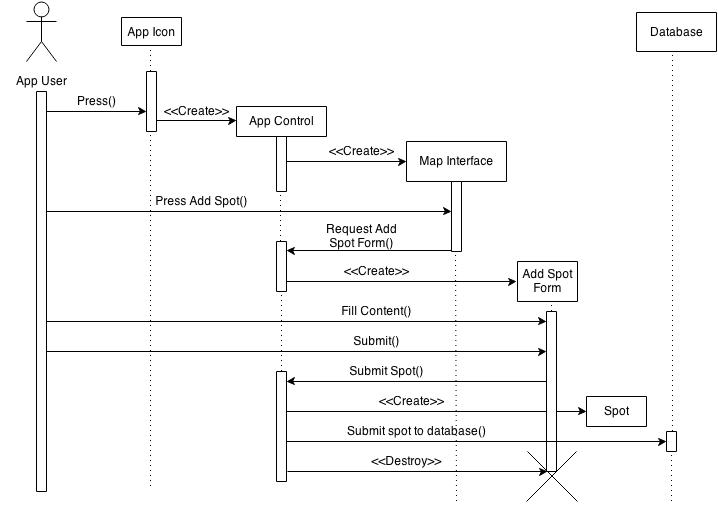
\includegraphics[scale = 0.5]{sekdia2}
\end{figure}

Brugeren starter App'en, ved at trykke på iconet for App'en, på sin telefon. App'en viser kort interfacen, 
som er et kort over brugerens nuværende position med en menu-bar i toppen. Brugeren vælger add spot fra menuen, 
ved at trykke på knappen markeret "Add Spot" i menu-baren. App'en viser en add spot formular, som er en række 
tekst-felter der skal udfyldes, samt en mulighed for at tilføje et billed. Brugeren udfylder formularen med spot 
informationerne og trykker på knappen markeret "Add" for at submite den. App'en sender spot-informationerne til databasen.

\newpage

\subsection*{Sekvensdiagram over indstillinger}
\begin{figure}[h]
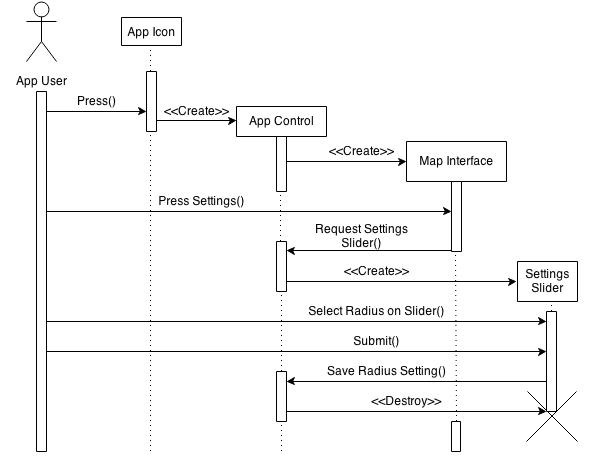
\includegraphics[scale = 0.5]{sekdia3}
\end{figure}

Brugeren starter App'en, ved at trykke på iconet for App'en, på sin telefon. App'en viser kort interfacen, 
som er et kort over brugerens nuværende position med en menu-bar i toppen. Brugeren vælger settings fra menuen, 
ved at trykke på knappen markeret med tandhjul i menu-baren. App'en viser en radius slider, som er en knap man kan hive i
for at indikere hvor lang en radius man vil loade spots fra. Brugeren vælger en radius, ved at hive knappen til den ønsket
radius og derefter trykke på knappen markeret "Accept" for at submite den. App'en gemmer den nye radius.

\pagebreak

\section{Systemdesign sammenfatning}

Vores plan vedrørende udviklingen af appen har indtil nu, været at bygge appen op i java med android developer tools. Det gav os en del udfordring, da vi ikke kunne få den simpleste udgave til at køre på en simulator. De mange timer og forsøg har gjort at vi følte os nødsaget til at gøre projektet mindre omfattende. 
\\\\
Derfor har vi valgt at bygge applikationen op webbaseret i html, css, javascript og mySQL, hvilket er programmer og metoder vi har erfaring med i forvejen. 
Hele implementeringen af Google maps foregår med javascript(altså som en hjemmeside), hvor vi så bagefter vil lave en android webview app, så vi kan tilføje applikationen på google play store. vi mangler at implementere alt andet end kortet på nuværende tidspunkt.\\\\
Vi arbejder med hjemmesidens server gennem en ftp via programmet filezilla. Serveren er bygget op med phpmyadmin og kører mySQL, dette bruger vi til at hente spots udfra databasen og derefter indsætte på kortet. Altså vi henter alt data udfra databasen som vi skal bruge til kortet. Til diverse funktioner vi har køres der forskellige queries i mySQL til at få de resultater ud som vi gerne vil have. Disse vil typisk være skrevet i PHP eller javascript.

\pagebreak

\section{Program- og systemtest}

Test af funktionaliteter gøres løbende internt i gruppen og dermed sikres det at funktionaliteterne gør det, de rent faktisk skal. Men derudover skal vi sikre ting som usability og performance, dette gøres f.eks ved hjælp af tænke højt øvelser.
\subsection*{Thinking out Loud}
Opgaver:\\\\
1. Åben appen og noter dig din egen lokation\\\\
2. Find det spot nærmest dig\\\\
3. Find information om spottet i fælledparken\\\\
4. Find en liste over alle spots\\\\
5. Find en butik\\\\
6. Tilføj et spot der hedder abc, med adressen xxx uden et billede\\\\
7. Ændrer afstanden i km for søgen af spots
\pagebreak
\subsection{Brugergrænseflade og interaktionsdesign}

\begin{figure}[ht]
\begin{minipage}[b]{0.45\linewidth}
\centering
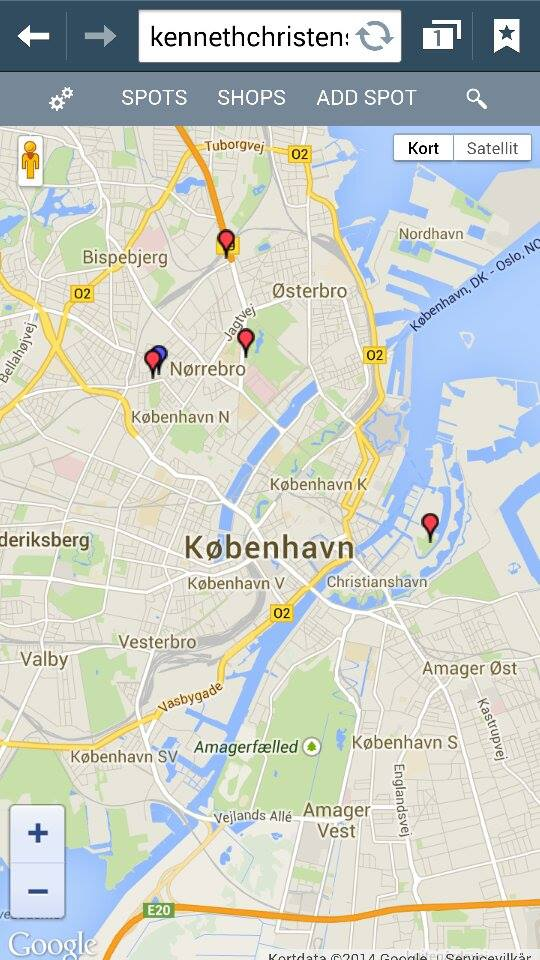
\includegraphics[width=\textwidth]{mobil1}
\caption{Startside}
\label{fig:figure1}
\end{minipage}
\hspace{0.5cm}
\begin{minipage}[b]{0.45\linewidth}
\centering
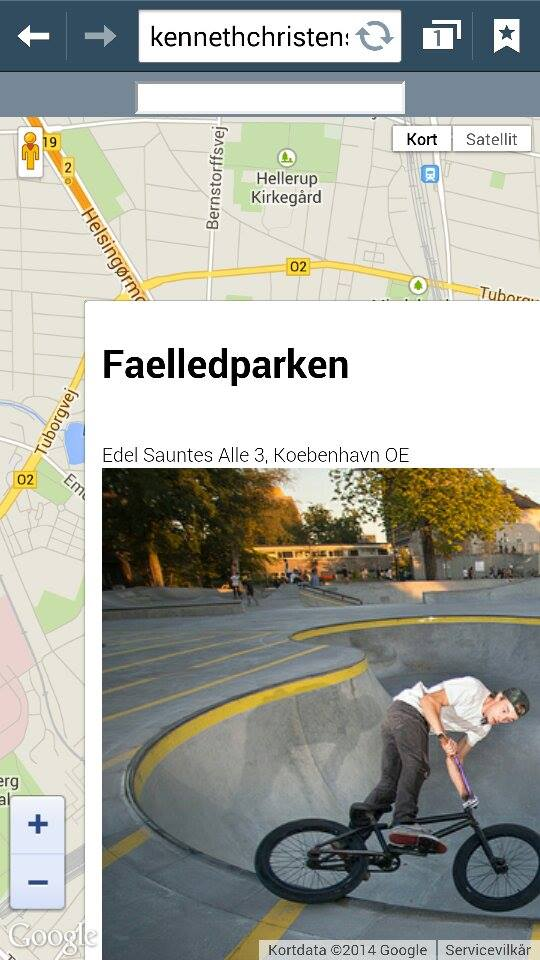
\includegraphics[width=\textwidth]{markers}
\caption{Markers}
\label{fig:figure2}
\end{minipage}
\end{figure}


\paragraph{Start side}\mbox{}\\
Dette er start siden af app'en. Her ses kortet med menuen i toppen. De røde markører viser kortet er spots og de blå viser butikker butikker.\\
\paragraph{Spot information}\mbox{}\\
Dette er overlayet med informationerne om et spot.\\ Det viser et billede af spottet og spottets addresse.

\newpage
\begin{figure}[ht]
\begin{minipage}[b]{0.45\linewidth}
\centering
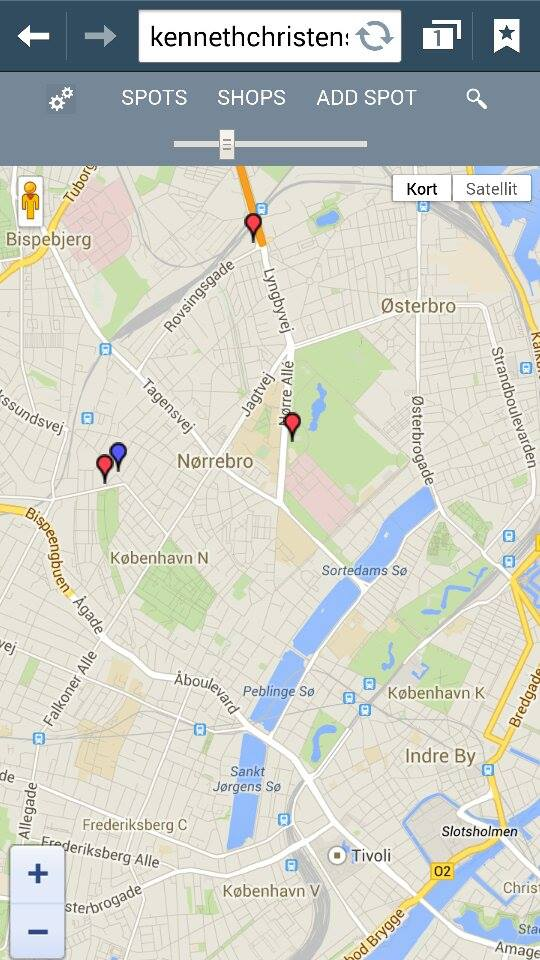
\includegraphics[width=\textwidth]{msettings}
\caption{Indstillinger}
\label{fig:figure3}
\end{minipage}
\hspace{0.5cm}
\begin{minipage}[b]{0.45\linewidth}
\centering
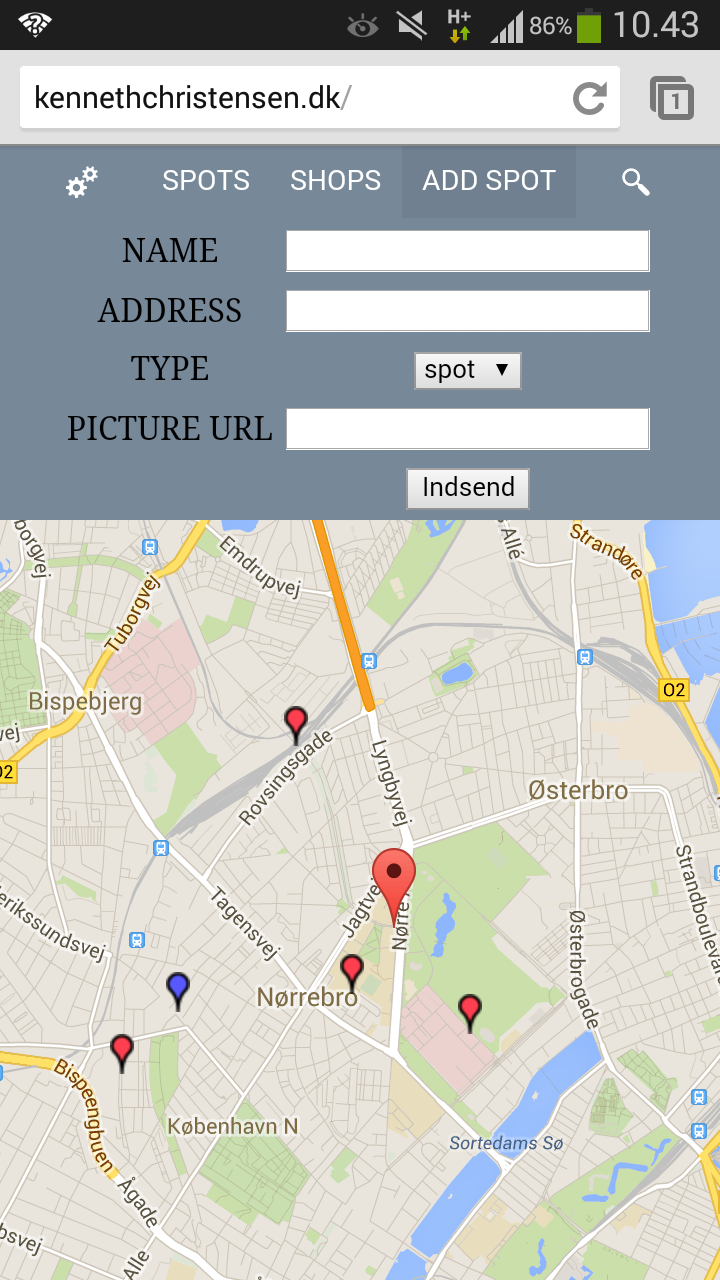
\includegraphics[width=\textwidth]{addspotscreen}
\caption{Add spot}
\label{fig:figure4}
\end{minipage}
\end{figure}



\paragraph{Indstillinger}\mbox{}\\
Dette er indstillingerne med slideren til radius for spotsne. Den er pt ikke implementeret men planen er at en skal kunne sætte en radius for langt man vil søge spots i udfra brugerens nuværende lokation.\\
\paragraph{Add Spot}\mbox{}\\
Her ses "Add Spot" funktionen som den vil se ud i appen. Den fungerer sådan at du indtaster et navn til dit spot, adressen, vælger hvilken type spot det er (spot/shop) og lader dig uploade et billede. Indsend sender formularen og ligger dit spot op i databasen.\\


\newpage
\begin{figure}[ht]
\begin{minipage}[b]{0.45\linewidth}
\centering
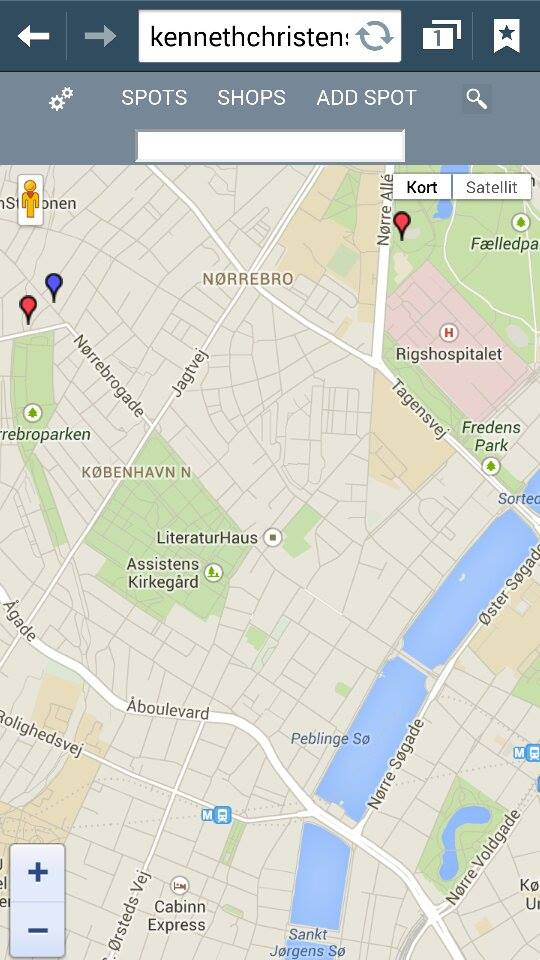
\includegraphics[width=\textwidth]{search}
\caption{Søg}
\label{fig:figure5}
\end{minipage}
\hspace{0.5cm}
\begin{minipage}[b]{0.45\linewidth}
\centering
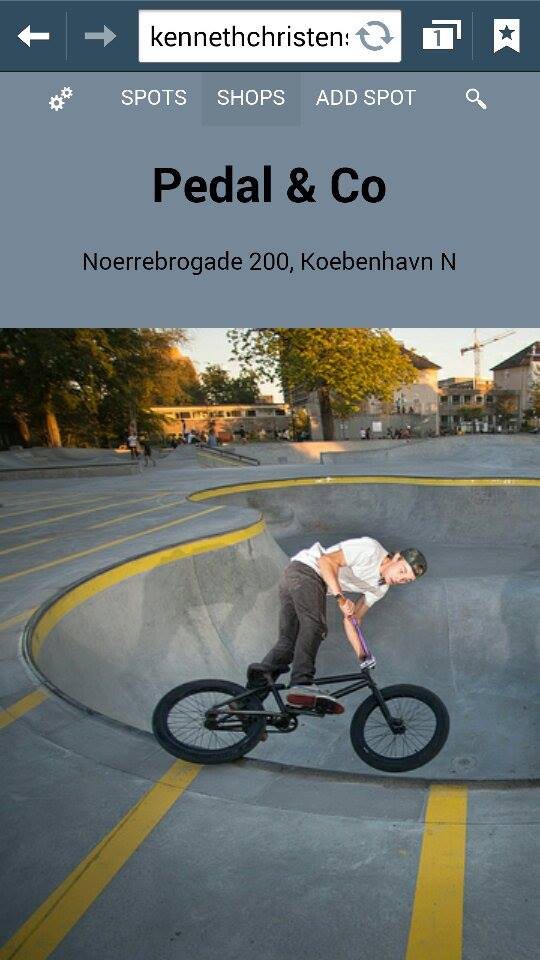
\includegraphics[width=\textwidth]{shops}
\caption{Shops}
\label{fig:figure6}
\end{minipage}
\end{figure}



\paragraph{Søg}\mbox{}\\
Dette er søgeboksen til at søge efter spot med, man søger på addresse. Efter man har søgt vil man blive vist en liste over de steder der passer til ens søgning. Fx. hvis man søger på et postnummer vil alle spots med det postnummer blive vist i en liste.\\
\paragraph{Butikker}\mbox{}\\
Denne minder meget om spots dog en kortere liste. Den viser listen over vores butikker, da det pt kun er 1 butik tilknyttet findes der kun en i databasen.\\

\newpage
\paragraph{Spots}\mbox{}\\
Dette er listen over spots. Den viser alle spots med deres billed og addresse.\\
\begin{figure}[h]
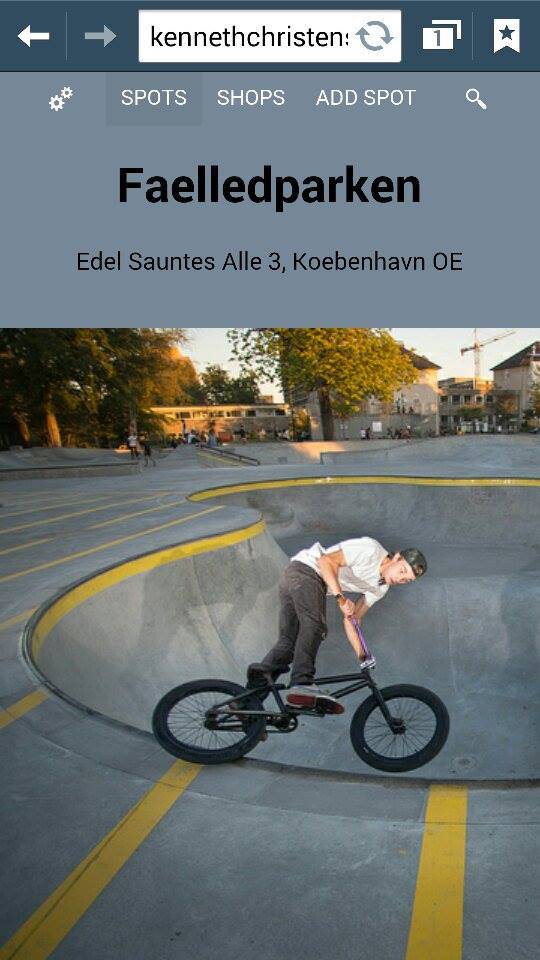
\includegraphics[scale = 0.3]{spot}
\end{figure}

\newpage
\paragraph{Flow-chart over skærmbilleder}\mbox{}\\
Dette er et flow-chart over vores skærmbilleder. Fra start siden kan man komme til alle de andre gennem et tryk i menuen eller på en marker på kortet. I søge funktion bliver man sendt videre til en liste over resultaterne af ens søgning.
\begin{figure}[h]
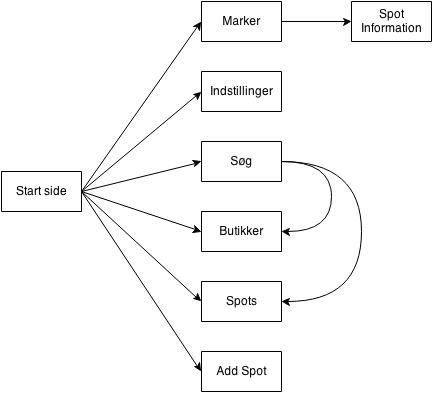
\includegraphics[scale = 0.8]{flowDiagram}
\end{figure}
\newpage
\subsection*{Youtube video}
\url{https://www.youtube.com/watch?v=0jjzZC0er9w&feature=youtu.be}
\subsection*{Resultat af Thinking out Loud}
\textbf{Testperson Damir:}
1. Vores test-person virkede lidt forvirret over hvad de forskellige markører var men fandt sin egen lokation ved den store markør.\\
2. Han finder hurtigt det spot der er tættest på sig selv og udtrykker sig om det er meget nemt at finde. Fanger ikke helt man kan trykke på spotsne til at starte med.\\
3. Han trykker nu på spottet og finder billedet og addressen på spottet.\\
4. Han tænker det umiddelbart må være der hvor der står spots. Han trykker på spots og får listen frem.\\
5. Hurtigt tænker han at han så må trykke på spots og derved få en liste frem og finder den ene butik i vores database. Han føler ikke at det er godt nok dokumenteret med de røde og blå markører.\\
6. Hurtigt videre og tilføjer det. Dog er der en fejl i vores link tilbage til hovedsiden så brugeren trykker derfor på tilbage kanppen.
7. Han virker lidt forvirret over hvor man skal. Han finder det dog til sidst under indstillinger.\\  \\
\textbf{Testperson Christoffer:}
1. Han finder hurtigt ud af han er ved den store røde "ting" som han kalder det.\\
2. Han kan ikke finde ud af hvad der er hvad så han trykker på røde og blå og finder ud af forskellen.\\
3. Han fandt løbehjulsparken som jo også ligger i fælledparken. Dog lå spottet for fælledparken også forkert på daværende tidspunkt.\\
4. Han trykker spots og kigger listen igennem. Han undrer sig over de spots der hedder abc med addresse xx men det er jo fra tidligere test. Han syntes topmenuen er lidt klodset.\\
5. Han trykker på shops og får listen som der inderholder pedal og Co. Han opfatter det er de blå der er shops men syntes godt det kunne være bedre forklaret.\\
6. Finder hurtigt knappen i menuen. Han syntes det er underligt at under add spot at man kan tilføje spot og shops. Han går derefter ind og finder det spot han har tilføjet i listen over spots.\\
7. Han finder det hurtigt under settings. Dog føler han igen det kunne være bedre forklaret.
\pagebreak
\section{Versionstyring}
Vi har fået opdateret vores hjemmeside 2 gange. Først den 31-05-2014 fra kennedc med commiten hjemmeside opdateret. Her havde vi fået lavet en søge funktion der tildels virkede. Derudover havde vi også fået ryddet op i vores database og den kan nu tage UTF-8.

Den næste commit der ændrer på vores projekt er fra den 03-06-2014 hvor hjemmesiden nu er stortset færdig.\\ Søge funktionen er nu blevet mere komplet og virker på postnumre, navn og addresse.\\\\
Derudover er der blevet lavet add spot, som gør det muligt for en bruger at tilføje deres eget spot til databasen. Både med og uden billede.\\\\
Vores største problem med de sidste opdateringer har været at få søge funktionen til at virke. \\\\
Dette har vist sig at være et større projekt en først antaget og vi har derfor, desværre, ikke kunne få denne implementeret korrekt dog er den stadig med da det var en original plan at den skulle være der og hvis vi skulle få lyst til at arbejde videre med det ved vi hvor vi skal starte. \\\\
Vores midlertidige projekt kan ses på \url{www.kennethchristensen.dk} Den burde nu stemme overens med vores rapporter og hvad vi har beskrevet.\\\\
Vores app til at kunne køre hjemmesiden på android er færdig.\\
Vi er ikke sikre på at den er kompatibel med at få en brugers position men dette vil altid blive et problem når nu den skal køre kunne køre offline.\\

\pagebreak
\section{Projektsamarbejdet}
Det interne arbejde i gruppen fungerer godt. Alle medlemmer i gruppen deltager aktivt, engageret og møder til tiden på de aftalte møde dage. Selve arbejdet prøver vi at fordele imellem os alt efter interesse og det sikrer en god stabil arbejds indsats.\\\\
 De dage vi mødes til "arbejdsdage" fungerer samarbejdet rigtig godt. Mere præcist vil det sige at vi er gode til at arbejde både selvstændigt og i mindre grupper og sørge for at alle mand er i gang. Sådan en arbejdsdag starter typisk med lidt planlægning og hvad vi skal nå, lidt snak om hvordan og hvem der skal lave hvad, hvorefter vi kommer i gang og stortset altid når dagens mål.\\\\
Vi har haft uventede problemer hvad angår systemdesignet da vi har måttet ændre kurs og gå over i en webbaseret udgave. Det har betydet at vi har haft nogle arbejdsspildtimer og vi er derfor ikke noget helt så langt som planlagt. Udover det, har flere funktioner voldet os problemer da vi måske teoretisk kunne løse dem, men har haltet lidt på implementeringen grundet erfaring. \\\\
I det vi tog skridtet fra android app til webbaseret app, har vi taget de første skridt i effektiviseringen. Derudover regner vi med at kunne begynde at arbejde selvstændigt på enkelte dele af systemet når vi har fået den første prototype helt op at køre. Det skullle bevirke at det bliver nemmere for de enkelte individer i gruppen at få plads i deres skema, til at få arbejdet på projektet og dermed få arbejdet flere timer. Udover det er det selvfølgelig vigtigt at sørge for at alle arbejder på det de har mest lyst til/er bedst til hvilket vil gøre de arbejder hurtigere og dermed mere effektivt.


\pagebreak
\section{Review}
\subsection*{Naur - Programming as Theory Building}

Abstractet til artiklen af Naur omkring "Programming as Theory Building" fra 1985 starter med at forklare essensen i hans artikel:\\\\
\textit{
"it is concluded that the proper, primary aim of programming is, not to produce programs, but to have the programmers build theories of the manner in which the problems at hand are solved by program execution"}\\\\
Den egentlige kode som programmørerne leverer, er ifølge Naur ikke den egentlige pointe i programmering. Da alt kode sandsynligvis hurtigt skal ændres igen. I stedet, må det virkelige mål for medlemmerne af et udviklingsteam, være at forstå, i dybden, det problem de forsøger at løse, og den løsning de udvikler til at løse det.\\\\
Hvis udviklings teamet opbygger en god teori, vil dennes software være bedre til at løse et givent problem og team medlemmerne vil finde det lettere at udføre de uundgåelige ændringer og forbedringer til sin software. Naur understreger at det er teorien der er vigtigst og at koden er uvæsentligt på en temmelig klar måde: Han hævder nemlig, at koden i isolation fra dens udviklere er død, selvom den stadig kan fungerer og producerer de resultater den skal.\\\\
\textit{"During the program life a programmer team possessing its theory remains in active control of the program, and in particular retains control over all modifications. The death of a program happens when the programmer team possessing its theory is dissolved. A dead program may continue to be used for execution in a computer and to produce useful results. The actual state of death becomes visible when demands for modifications of the program cannot be intelligently answered. Revival of a program is the rebuilding of its theory by a new programmer team"}\\
\newpage
\noindent I forhold til vores projekt og erfaringer med problem løsning indtil videre, kan det være svært at være uening i Nauers holding. Det er først når man for alvor har forstået et problem at man er i stand til at komme med en god løsning. Det viser sig tydeligt når vi ser på kode vi selv har skrevet kontra det andre har skrevet. Vores egen vil altid virke mere overskuelig og det vil være nemmere at rette og udvikle på. Modsat andres kode der som oftest vil være forvirrende og uoverskuelig. Hvilket i høj grad må skyldes niveauet af forståelse, for det givne problem koden skal løse, det er nemlig først når man forstår problemet at man forstår løsningen. Men det vil immervæk uanset hvad, være sværere at komme med gode inteligente løsninger, når man ikke selv har været med under hele processen og dermed kunne man godt konstatere "koden er død".
\newpage
\subsection*{The M.A.D. Experience: Multiperspective Application Development in evolutionary prototyping.}

Artiklen handler om de erfaringer et udviklingshold gjorde sig i sammearbejde med et skipsfragt-firma da de skulle udvikle et system for dem. Forfatterne forklarer i introduktionen om samarbejdet med firmaet, om hvilke forhindring som opstod og hvad de lærte af processen. De fremhæver selv 3 ting som de vigtigste de vil argumentere for.\\\\
1: Analysis is more than finding nouns and verbs.\\
Hvor de vil argumentere for at det ofte kan være nødvendigt og ligefrem brugbart, at basere sin analyse på mere advanceret metoder end de normalt anvendte. Så som en ethnografisk analyse af den sociale organisation på arbejdspladsen. Dvs en dybdegående gennemgang af hvordan arbejdet foregår uden analytikerens bias påvirker analysen.\\
2: Design is more than filling in details in the Object-Oriented analysis model.\\
Hvor de vil argumentere for at det er nødvendigt og brugbart at bruge teknikker fra sammenarbejds design-processer. Altså hvor designere og brugere arbejder tæt sammen i design fasen, med f.eks. mock-ups til at formulere konkrete design-løsninger og hvordan de kan bruges i praksis.\\
3: Implementation is more than translating design models into code.\\
Hvor de vil argumentere for at  det er vigtigt at starte med at implementere tidligt i processen. Da implementationen kan medføre ændringer og den oprindelige design model højst sandsynligt vil ændre sig når implementeringen starter. Feedback fra den tidlige implementation vil også påvirke projekt fremad og det vil derfor være en fordel at ha feedbacken tidligt i processen.\\\\
Artiklen går herefter meget i detajler om selve projektet som blev udarbejdet med skibsfragt-firmaet. Og til sidst konkludere forfatterne så på deres erfaringer. De laver en punktvis gennemgang af deres 3 tidligere fremhævet argumenter, og kommer med en kort forklaring på hvorfor deres tidligere argumentation holder vand i deres tilfælde.
\newpage
Det vi i gruppen synes vi kan tage med fra artiklen er noget begrænset da det handler om et meget specifik projekt som ikke rigtigt relatere til vores eget, og derfor er det egenligt kun de tre opstillet punkter som der rigtigt kan tages i betragtning. Vigtigheden af en god analyse af det arbejdsmiljø projekt skal bruges i fremover er klart en ting at tage med fra artiklen, som ville kunne hjælpe i vores fremtidige projekter. En anden klar ting at medtage er det man involverer de fremtidige bruger i design-processen og begynder implementation tidligt, for at løbende kunne lave gavnlige ændringer til projektet.
\pagebreak
\section{Litteratur}
\begingroup
\renewcommand{\section}[2]{}%
%\renewcommand{\chapter}[2]{}% for other classes
  \begin{thebibliography}{1}
  \bibitem{Bog} Bruegge, Bernd and Dutoi, Allen H.{\em Object-Oriented Software Engineering Using UML, Patterns, and Java. Third Edition}  2010.

  \bibitem{OOAD}  L. Mathiassen, A. Munk-Madsen, P. A. Nielsen and J. Stage. {\em Object-Oriented Analysis and Design kap 1} 2000

  \bibitem{Scrum} Sutherland, Jeff {\em Scrum Handbook} ?
  
  \bibitem{EP} Highsmith, Jim {\em Extreme Programming} 2000 Cutter Consortium

  \bibitem{Silverbullet} Brooks {\em No Silver Bullet
  } 1986

  \bibitem{Mock} Kyng, Morten and Ehn, Pelle {\em Mocking-it-up} 1991
  
  \bibitem{TA} Molich, Rolf{\em User Testing, Discount User Testing} 2003

  \bibitem{Coop} Frøkjær, Erik and Hornbæk, Kasper {\em Cooperative Usability Testing} 2005
  
  \bibitem{Fake} Parnas, David Lorge and Clements, Paul C {\em A Rational Design Process...How and Why to Fake IT} 1986
    
  \bibitem{Naur} ? {\em Naur Programming As Theory Building} 1985
      
  \bibitem{MAD} Michael Christensen, Andy Crabtree, Christian Heide Damm, Klaus Marius
Hansen, Ole Lehrmann Madsen, Pernille Marqvardsen, Preben Mogensen, Elmer
Sandvad, Lennert Sloth, Michael Thomsen {\em The M.A.D. experience} 1998
   
  \bibitem{Design} Gould, John D. and Lewis, Clayton {\em Designing for Usability:
Key Principles and
What Designers Think} 1985

  \bibitem{Must} Bødker, Kensing and Simonsen {\em The must book Kap. 9} 2004
      
  \bibitem{UX} Klein, Laura {\em UX for Lean Startups} 2013
            
  \bibitem{Testing} Sestoft,Peter  {\em Systematic Software Testing} 2008
      
  \end{thebibliography}
  \endgroup
\section{Bilag}

\subsection*{Commitlog}
* <6015312> 2014-06-03 [mhejselbak]  (HEAD, origin/master, origin/HEAD, master) Tilføjet Think-aloud \\
* <5d3b60b> 2014-06-03 [kennedc]  Hjemmeside næsten færdig \\
* <c2994f9> 2014-06-03 [runefranch]  gennemgang af rapport \\
* <6dcd2a0> 2014-06-03 [runefranch]  Tilføjet flowchart med tekst\\
* <83c5854> 2014-06-03 [rasmus03]  Tilføjede addspot screenshot\\
* <30d072f> 2014-06-03 [rasmus03]  Opdaterede dele i delrapporten\\
* <bbecb80> 2014-06-03 [runefranch]  tilføjet review\\
* <e9f679d> 2014-06-02 [mhejselbak]  Udvidet forklaringer af billeder\\
* <81b1a02> 2014-06-02 [rasmus03]  Tilføjede review af Programming as Theory Building til delrapport 4\\
* <cba1e23> 2014-05-31 [kennedc]  Hjemmeside opdateret\\
* <4ddf0c1> 2014-05-28 [rasmus03]  ups\\
* <84685aa> 2014-05-28 [runefranch]  tilføjet billed og txt\\
* <05dfe3f> 2014-05-28 [runefranch]  ups\\
* <9617401> 2014-05-28 [rasmus03]  Billeder til mockup\\
* <0c23f3a> 2014-05-28 [rasmus03]  nyt mobil billede\\
* <80dac95> 2014-05-28 [rasmus03]  Opdaterede punkt 5\\
* <1efffc2> 2014-05-28 [rasmus03]  Tilføjede mere tekst overall\\
* <f7c9279> 2014-05-28 [mhejselbak]  Tilføjet litteratur\\
* <94a805e> 2014-05-28 [rasmus03]  Rettede til et rigtige billede i USM\\
* <80972ed> 2014-05-28 [rasmus03]  Use case model: mere test\\
* <ef6a0d9> 2014-05-28 [runefranch]  tilføjet beskrivelser\\
* <c79a247> 2014-05-28 [rasmus03]  Små fejlrettelser\\
* <3aad81a> 2014-05-28 [rasmus03]  Opdateret PDF\\
*   <08d758e> 2014-05-28 [mhejselbak]  Merge branch 'master' of https://github.com/mhejselbak/PKSU\\
|\textbackslash \\ 
* | <5f70296> 2014-05-28 [mhejselbak]  FK og IFK\\
| * <b95bc9c> 2014-05-28 [rasmus03]  Tilføjede ny use case model \\
|/  \\
* <fdb8b22> 2014-05-28 [rasmus03]  Klasse diagram tekst\\
* <f306564> 2014-05-28 [rasmus03]  oprydning\\
* <fabd1cd> 2014-05-28 [rasmus03]  Mobil billede\\
* <075fbeb> 2014-05-28 [rasmus03]  Tilføjede første udkast til delrapport 4\\
* <c92cac7> 2014-05-28 [mhejselbak]  clase diagram added\\
* <0cb3d7d> 2014-05-15 [runefranch]  lidt redigering\\
* <a51efd6> 2014-05-14 [rasmus03]  Opdaterede små fejl i delrapport 3: klar til aflevering \\
* <84609b5> 2014-05-14 [rasmus03]  Ingen ændringer blot opdateret PDF’en \\
* <60d2678> 2014-05-14 [runefranch]  delrapport 3 opdate v2 \\
* <4cf2d0d> 2014-05-14 [runefranch]  delrapport 3 opdate\\
* <b5e97ea> 2014-05-14 [rasmus03]  Review af “Silver Bullet” \\
*   <e963633> 2014-05-14 [mhejselbak]  Merge branch 'master' of https://github.com/mhejselbak/PKSU\\
|\textbackslash \\
* | <aa8f509> 2014-05-14 [mhejselbak]  delrapport3 opdateret v3\\
* | <9f9797c> 2014-05-14 [mhejselbak]  delrapport3 opdateret v2\\
| *   <6df32c0> 2014-05-14 [kennedc]  Merge branch 'master' of https://github.com/mhejselbak/PKSU\\
| |\textbackslash  \\
* | | <192e6af> 2014-05-14 [mhejselbak]  delrapport3 opdateret \\
* | | <192e6af> 2014-05-14 [mhejselbak]  delrapport3 opdateret \\
* | | <73f7798> 2014-05-14 [mhejselbak]  delrapport 3 tilføjet\\
* | | <8fff4f0> 2014-05-14 [mhejselbak]  delrapport 3 tilføjet\\
| |/  \\
|/|   \\
* | <a9c842d> 2014-05-08 [rasmus03]  Genupload af delrapport\\
* | <d58b7ea> 2014-05-08 [mhejselbak]  Delrapport 2 genafl tilfoejet\\
* | <2572462> 2014-05-08 [rasmus03]  Tilføjede en ny usecasemodel\\
* | <04acdab> 2014-05-07 [rasmus03]  Mindre opdateringer til delrapport 2 - intet nyt\\
| * <8fe6d52> 2014-05-07 [kennedc]  html og css\\
|/  \\
* <533b5cb> 2014-05-07 [mhejselbak]  added more to part 5\\
* <c5d6de6> 2014-05-07 [runefranch]  updateret delrapport\\
* <c4bdcc5> 2014-05-07 [rasmus03]  Opdaterede delrapport 2 med nye sekvensdiagrammer\\
* <e4f926b> 2014-05-07 [rasmus03]  Tilføjede gruppe reviews (igen)\\
*   <a8c5bbd> 2014-05-07 [runefranch]  Merge branch 'master' of https://github.com/mhejselbak/PKSU\\
|\textbackslash \\  
* | <95229b4> 2014-05-07 [runefranch]  Sekvens diagram \\
| * <d3ad6bd> 2014-05-07 [rasmus03]  Flyttede log.log til den rette mappe \\
|/  \\
* <a0eb8ab> 2014-05-07 [mhejselbak]  Deleted style.css and edited delrapport2 \\
* <3db9ac0> 2014-05-07 [rasmus03]  Opdaterede tekst i delrapport 2\\
* <b4614f0> 2014-04-28 [mhejselbak]  CSS til hjemmeside\\
* <d0c4133> 2014-04-28 [rasmus03]  Tilføjede første udlæg til den webbaserede android application - Ingen test af funktioner muligt\\
* <ba05d40> 2014-04-28 [rasmus03]  Tilføjede vores review af “Mood”\\
* <1da40ab> 2014-04-24 [rasmus03]  Updaterede filer til delrapport 2\\
* <89ae7a4> 2014-04-24 [rasmus03]  Commitlog billede\\
* <6f57d2e> 2014-04-24 [rasmus03]  Tilføjede vores udkast til hjemmesiden - Ingen implementeringer\\
* <2077057> 2014-04-24 [runefranch]  Nyt sekvens diagram\\
* <a006ca4> 2014-04-24 [runefranch]  sidste sekvens diagram\\
* <f2ad5a2> 2014-04-23 [rasmus03]  Updated files and added screenshots\\
* <c201cd9> 2014-04-23 [runefranch]  sekvens diagram\\
* <ee33ad2> 2014-04-23 [rasmus03]  Opdaterede delrapport2 med 2/2 review og use-cases. Standard clean up af unødige filer.\\
* <592de43> 2014-04-23 [runefranch]  reviewartikel \\
* <e77b576> 2014-04-23 [rasmus03]  FACTOR model - Bruges i delrapport 2\\
* <599276d> 2014-04-23 [rasmus03]  Delrapport 2 - Består af punkt 1, 2 og 1/2 review\\
* <b2271ec> 2014-04-22 [mhejselbak]  Prototype\\
* <6e1b71b> 2014-04-10 [runefranch]  review update\\
* <d81beae> 2014-04-09 [runefranch]  Review\\
* <19705bc> 2014-04-03 [mhejselbak]  Initial commit\\
\subsection*{Referat fra sidste møde med kunde}
Møde med Travis den 8/6 \\
Vi mødtes med travis i bmxbutikken eller som deres butik på nørrebrogade hedder "pedal \& Co" Her fremviste vi vores program til ham og snakkede om forbedringer og evt ekstra funktionalitet, vi diskuterede også hvilken slags spots der skulle op og om man evt. skulle holde nogle spots hemmelige for brugerene for at ikke opfordre små børn til at hoppe over hegn f.eks.\\
Han var rigtig tilfreds med resultatet af programmet indtil videre, og glædede sig til at det blev færdig, så han kunne få det ud til den danske bmx scene. Han havde dog også nogle ting, som han synes vi skulle tænke ekstra over. Han synes bla. ikke at hjemmesiden var helt inuitiv nok han kom med et eksempel med den lille gule mand og google street view, hvor at en erfaren bruger af google maps ved at man skal trække den gule mand ned på kortet, vil en bruger der ikke er vand til google maps ikke kende den funktionalitet. Derfor ville han gerne have en knap inde i infowindows med streetview, så en bruger af appen også trykke på en knap indei  infowindowet og se googles billeder af spottet.\\
Derudover snakkede vi også om at få brugere til at bruge hjemmesiden, hvor vi blev enige om at det var vigtigt at starte med en database med en del spots, simpelthen for at få brugerne til at bruge hjemmesiden. Derudover hvis der først er brugere på siden vil de forhåbentlig også selv uploade deres egne lokale spots og på den måde kan spotguiden udvide sig til at være national, da der kommer massere af bmx'ere og skatere fra Jylland til hovedstaden for at køre
\end{document}